\documentclass[twocolumn, letter, 10pt, landscape]{article}
\usepackage[fontsize=8pt]{scrextend}
\usepackage{graphicx}
\usepackage{enumitem}
\usepackage{pifont}
\usepackage{fontspec}
\usepackage[T1]{fontenc}
\usepackage[utf8]{inputenc}
\pagestyle{empty}
\setlength{\parindent}{0pt}
\usepackage[left=0.2in,top=0.2in,right=0.2in,bottom=0.3in]{geometry}
\graphicspath{{./images/}}
\usepackage{sectsty}
\usepackage{titlesec}
\usepackage{amssymb}
\usepackage{amsmath}

\sectionfont{\fontsize{10}{15}\selectfont}
\titlespacing*{\section}{0pt}{0pt}{0pt}
\titlespacing*{\subsection}{0pt}{0pt}{0pt}
\newcommand{\mb}{\mathbf}
\newcommand{\tb}{\textbf}
\newcommand{\ti}{\textit}
\newcommand{\bms}{\begin{bmatrix}}
\newcommand{\bme}{\end{bmatrix}}
\newcommand{\bit}{\vspace{-0.1in}\begin{itemize}\setlength\itemsep{-0.05in}}
\newcommand{\eit}{\end{itemize}\vspace{-0.1in}}
\newcommand{\ben}{\vspace{-0.1in}\begin{enumerate}\setlength\itemsep{-0.05in}}
\newcommand{\een}{\end{enumerate}}
\newcommand{\mal}{\mathcal{L}}
\newcommand{\re}{\mathbb{R}}
\newcommand{\derv[3]}{\frac{\partial {#2}}{\partial {#3}}}
\newcommand{\grad[3]}{\nabla_{#2}{#3}}
\newcommand{\ex}{\mathbb{E}}
\newcommand{\vt}{\text}
\newcommand{\eps}{\epsilon}
\setcounter{section}{1}

\begin{document}

\textbf{Kalon Lucas Kelley - 406039396}

\section{Lecture 2}
\textbf{Supervised} learning, we will be given data points $x^{(i)}$ that come with an associated label $y^{(i)}$ which tells us in a classification problem what type of image x is or what value we want to map x to in a regression problem.

\textbf{Classification:} $y^{(i)}$ represent classes or categories that $x^{(i)}$ may belong to. e.g. in CIFAR-10 we are given a bunch of images $\mathbf{x}$ which are $32\times 32 \times 3$ (tensor) and each image $\mathbf{x}$ will be associated with one label $y$ which there are 10 of. Given an image $\mathbf{x}$ determine which of the 10 classes it belongs to.

Reshape the tensor into a vector $32\times 32\times 3 = 3072$ meaning $\mathbf{x}\in \mathbb{R}^{3072}$

Want to define some function $class\leftarrow f(\mathbf{x})$ takes the input image and returns the class the image belongs to.

Because were given pairs of images and labels to train on this is called \textbf{supervised}

\subsection{Regression}
\textbf{Regression} doesn't predict a class but produces a number at the output.

e.g. We want to rent a home in westwood and we are trying to find a relationship between square footage and monthly rent. We want to predict what they rent will be given the square footage and the rent isn't a class it is a real dollar amount hence why this is a \textbf{regression} problem and \textbf{not classification}.

In machine learning our goal is to learn some function $f(sq\:ft) \rightarrow rent$ that takes the square footage and produces the rent.

We have to define what model we are going to use, the model of $f$. (e.g. $ax+b$) because if we look at the data graphically it may look like they are pretty well described linearly.

$y = ax+b$ where \textbf{y} is the monthly rent and \textbf{x} is the square footage. And both y and x are given to us by data where a and b are knobs we get to tune to get this model to fit as best as possible \textbf{hyperparameters}

We could use a different model for $f$ like $b+a_{100}x^{100} + a_{99}x^{99}+...+a_1x$ in which case we have many more parameters to tune and can fit the data perfectly but this leads to \textbf{overfitting} because the model becomes much worse at generalization.

Later on our $f$ model will be a neural network.

\textbf{How do we assess how good our model is:}\\
inputs: $x^{(i)}$ (i is for indexing over all inputs)\\
outputs: $y^{(i)}$\\
$\hat{y}^{(i)}=b+ax$ we can tell one model is better than another by checking if $\hat{y}^{(i)}$ of a given model is closer than the true outputs $y^{(i)}$

We define some error $\epsilon_i = y^{(i)}-\hat{y}^{(i)}$ if we want to quantify how good a model is we look for the model with the smallest error.

\textbf{Loss Function:} is a function which tells us \textbf{quantitatively} how good or how bad our model is $\mathcal{L}$ also sometimes called a cost function.

$\mathcal{L} = \sum_{i=1}^{N} (y^{(i)}-\hat{y}^{(i)})$ the problem with this is that sign is not considered meaning if a data point resides below the prediction and another one resides equally above the prediction their errors will cancel out in the summation making the loss seem like $0$. Instead we use the squared error as follows $\mathcal{L} = \sum_{i=1}^{N} (y^{(i)}-\hat{y}^{(i)})^2$ and oftentimes this is normalized by $\frac{1}{2}$ because we integrate and this allows the square to cancel. It is also normalized by $N$ so this becomes the average loss per example. $\mathcal{L} = \frac{1}{2N}\sum_{i=1}^{N} (y^{(i)}-\hat{y}^{(i)})$. Strictly speaking these constants are not necessary but helpful.

\textbf{Why not absolute value?} you don't get an analytic solution which can be derived by hand but this can still be optimized through gradient descent. Also the squared error magnifies larger distances meaning further away points make loss very bad.

\textbf{Re-writing more mathematically}\\
$\hat{y}=ax+b$ where $a$ and $b$ are parameters we get to choose to make the model as good as possible

$\hat{y} = \theta^T\hat{\mathbf{x}}$ where $\theta = \begin{bmatrix} a\\b\end{bmatrix}$ and $\hat{\mathbf{x}} = \begin{bmatrix} x \\ 1 \end{bmatrix}$

The 1 is added to $\hat{\mathbf{x}}$ to ensure $b$ is a bias added at the end

\textbf{Cost Function}
$\mathcal{L}(\theta) = \frac{1}{2}\sum_{i=1}^N(y^{(i)}-\hat{y}^{(i)})^2 = \frac{1}{2}\sum_{i=1}^N(y^{(i)}-\theta^T\hat{\mathbf{x}}^{(i)})^2$ leaving out the normalizing factor of $N$ because it doesn't make a functional difference in getting to the optimum.

When $\mathcal{L}$ is larger the model is worse meaning we want to minimize $\mathcal{L}$ which is an optimization problem so we must calculate $\frac{\partial\mathcal{L}}{\partial\theta}$ for our simple example $\mathcal{L}(\theta)$ is a quadratic function of theta (parabola) so there is only one minima which is global. \textbf{With neural networks the loss landscapes are much more complicated and countless minima and maxima}

\subsection{Vector \& Matrix Derivatives}
Typically call these derivatives gradients. We have the following syntax $y$ (math notation no bold) is a scalar, $\mathbf{y}$ bold lowercase is a vector, and $\mathbf{Y}$ is a matrix or tensor.

Differentiate a scalar $y$ w.r.t a vector $\mathbf{x}$

$\frac{\partial y}{\partial \mathbf{x}} = \nabla_{\mathbf{x}}y$ e.g. with a scalar $y$ and vector $\mathbf{x} \in \mathbb{R}^n$ then $\nabla_{\mathbf{x}}y = \begin{bmatrix} \frac{\partial y}{\partial x_1} \\ \frac{\partial y}{\partial x_2} \\ \vdots \\ \frac{\partial y}{\partial x_n} \end{bmatrix}$ we know that the derivative of a scalar with respect to a scalar tells us ho much moving the second one will move the first. (e.g. $\Delta y$ due to $\Delta x_1$ is $\approx \frac{\partial y}{\partial x_1}\Delta x_1$ if $\frac{\partial y}{\partial x_1} = 0.5$ and we change (wiggle) $x_1$ by $0.01$ then we would expect $\Delta y \approx 0.005$

What we can now do $\Delta y \approx \sum_{i=1}^n\frac{\partial y}{\partial x_i}\Delta x_i$ which can be written as a \textbf{dot product} telling us concisely how $y$ will change when we wiggle a vector $\mathbf{x}$

$\Delta y \approx (\nabla_{\mathbf{x}}y)^T\Delta\mathbf{x}$ which generalizes derivative concepts from calculus to vectors. Think of this as how changing our \textbf{parameters} changes our \textbf{loss}

\textbf{Example:}

If $y = \theta^T\mathbf{x} = \theta_1x_1 + \theta_2x_2 + ... + \theta_nx_n$ then $\nabla_\mathbf{x}y = \begin{bmatrix} \theta_1 \\ \theta_2 \\ \vdots \\ \theta_n \end{bmatrix} = \theta$

\textbf{Another example:}
if $f(x) = \mathbf{x}^T\mathbf{A}\mathbf{x}$ what is $\nabla_{\mathbf{x}}f(x)$

$\mathbf{A} = \begin{bmatrix} a_{1,1} & a_{1,2} & ... & a_{1,n} \\
  a_{2,1} & a_{2,2} & ... & a_{2,n}\\
  \vdots & \vdots & & \vdots \\
  a_{n,1} & a_{n,2} & ... & a_{n,n}
\end{bmatrix}$ We can re-write the product in summation form as\\
$\sum_{i=1}^{n}\sum_{j=1}^{n} x_i \times a_{i,j} \times x_j$ and now differentiate each term as follows

$\frac{\partial f(x)}{\partial x_1} = 2a_{1,1}x_1 + \sum_{j=2}^{n}a_{1,j}x_j + \sum_{i=2}^{n}a_{i,1}x_1$ because those are all the terms which can contain an $x_1$ this can be repeated for all $x_i$ and this can even be simplified further by putting the first term into the second two as follows. $\frac{\partial f(x)}{\partial x_1} = \sum_{j=1}^{n}a_{1,j}x_j + \sum_{i=1}^{n}a_{i,1}x_1$ which can be written in matrix sum notation as $(\mathbf{A}\mathbf{x})_1 + (\mathbf{A}^T\mathbf{x})_1$ and we can put all of these elements for all $x_i$ into a vector for the final gradient $\nabla_{\mathbf{x}}f(x) = (\mathbf{A}+\mathbf{A}^T)\mathbf{x}$ and in the case where $\mathbf{A}$ is symetric this is equivalent to $2\mathbf{Ax}$.

This can be sanity checked by assuming $n=1$ in which case all our terms are scalars and we know that $\frac{\partial ax^2}{\partial x} = 2ax$

\textbf{Matrix Derivatives:} If $\mathbf{A}\in \mathbb{R}^{m\times n}$ then $\nabla_{\mathbf{A}}y \in \mathbb{R}^{m\times n}$ where each element is the derivative of y w.r.t the same element of the matrix.

We can no go back and rewrite the loss function (cost function) as follows

$\mathcal{L}(\theta) = \frac{1}{2}\sum_{i=1}^N(y^{(i)}-\theta^T\hat{\mathbf{x}}^{(i)})^2 = \frac{1}{2}\sum_{i=1}^N(y^{(i)}-\theta^T\hat{\mathbf{x}}^{(i)})^T(y^{(i)}-\theta^T\hat{\mathbf{x}}^{(i)})$

Where we can reorder the $\theta^T\hat{\mathbf{x}}^{(i)}$ by applying a transpose becoming $(\hat{\mathbf{x}}^{(i)})^T\theta$ then vectorize it to remove the summation.

\subsection{Denominator vs Numerator layout}
\textbf{Denominator layout:} $\mathbf{A}\in \mathbb{R}^{m\times n}$ then $\nabla_{\mathbf{A}}y \in \mathbb{R}^{m\times n}$ and $\mathbf{x}\in \mathbb{R}^{n\times 1}$ then $\nabla_{\mathbf{x}}y \in \mathbb{R}^{n\times 1}$

\textbf{Numerator layout:} $\mathbf{A}\in \mathbb{R}^{m\times n}$ then $\nabla_{\mathbf{A}}y \in \mathbb{R}^{n\times m}$ and $\mathbf{x}\in \mathbb{R}^{n\times 1}$ then $\nabla_{\mathbf{x}}y \in \mathbb{R}^{1\times n}$

They are the exact same values between numerator and denominator but just transposed.

\section{Lecture 3}
Our re-written loss function from lecture 2 vectorized $\mathcal{L}=\frac{1}{2}(Y-\mathbf{X}\theta)^T(Y-\mathbf{X}\theta)$ where $Y \in \mathbb{R}^N$ and is the vector of all $y^{(i)}$, $\mathbf{X}\in \mathbb{R}^{N\times 2}$ and is the vector of vectors $\hat{\mathbf{x}}^{(i)^T}$

$\mathcal{L}(\theta)=\frac{1}{2}(Y^TY-Y^T\mathbf{X}\theta - \theta^T\mathbf{X}^TY + \theta^T\mathbf{X}^T\mathbf{X}\theta) = \frac{1}{2}(Y^TY-2Y^T\mathbf{X}\theta + \theta^T\mathbf{X}^T\mathbf{X}\theta)$

Recall $\frac{\partial \mathbf{z}^T\theta}{\partial\theta} = \mathbf{z}$ and we'll say $Y^T\mathbf{X} = \mathbf{z}^T$ and using $\nabla_\theta(\theta^T \mathbf{A}\theta) =(\mathbf{A} + \mathbf{A}^T)\theta$ where $\mathbf{A} = \mathbf{X}^T\mathbf{X}$

$\frac{\partial\mathcal{L}(\theta)}{\partial\theta} = \frac{1}{2}(0-2\mathbf{X}^TY + (\mathbf{X}^T\mathbf{X}+\mathbf{X}^T\mathbf{X})\theta) = -\mathbf{X}^TY + \mathbf{X}^T\mathbf{X}\theta$ then setting that to 0 and solving we get

$\theta = (\mb{X}^T\mathbf{X})^{-1}\mathbf{X}^TY$ and this is \textbf{Least Squares}

$\mb{X}^T\mb{X}\in \mathbb{R}^{2\times 2}$ if we have more features than samples then $\mb{X}^T\mb{X}$ will not be invertable so we cannot use the same formula for $\theta$

\subsection{Least Squares for Higher Order Polynomials}
We can use the same math as before for higher order polynomials with $\hat{\mb{x}} = \bms x^n \\ x^{n-1} \\ \vdots \\ x \\ 1 \bme$ and $\theta = \bms a_n \\ a_{n-1} \\ \vdots \\ a_1 \\ b \bme$ where our polynomial is $y=b+a_1x+a_2x^2+...+a_nx^n$ leaving our same equation $\theta^T\hat{\mb{x}}$

\textbf{A higher degree polynomial will \textit{always} fit the provided data as well as a lower order polynomial or better}

\subsection{Overfitting}
If we make the order of the polynomial higher we will fit the data better but may not be as good at generalizing, we don't care about how well it fits our training data but how well it is able to generalize on new unseen data.
\bit{}
\item
  \tb{Training Data:} data that is used to learn the parameters of your model
\item
  \tb{Testing Data:} data that is excluded in training and used to score your model (unseen)
\eit{}
Overfitting occurs when a model has very low training error but high testing error (does not generalize) lots of data helps to mitigate overfitting even with higher order polynomials. (When lots of data is available we will be able to use more complex models)

\subsection{Underfitting}
Making a model \ti{overly simple} will underfit the data meaning the model has both a high training and testing error not generalizing or fitting the training data well at all. This is because the model is not expressive enough.

\subsection{Hyperparameters}
Things we choose beforehand that have to do with the model itself (like the order of the polynomial) and these hyperparameters can have a profound affect on the model fitting.

\subsection{Data Sets}
There are 3 types of data sets or partitions which we need for creating a model.
\bit
\item \tb{Training Data:} Data that is ued to learn the parameters of your model
\item \tb{Validation Data:} Data that is used to optimize the hyperparameters of your model, avoiding the potential of overfitting to a nuanced dataset
\item \tb{Testing Data:} Data that is used to score the final model after all optimizations
\eit

\subsection{K-fold Cross Validation}
Assuming we have a \tb{separate} testing set, to train the model a common approach is k-fold cross validation which is used as follows.
\bit
\item Let the training dataset contain $N$ examples (e.g. 800)
\item Split the data into $k$ equal sets containing $\frac{N}{k}$ examples each each of which is called a fold
\item $k-1$ folds are datasets used for training the model parameters (e.g. 3 folds 600 examples) for $\theta$
\item The remaining fold is a \tb{validation} dataset used to evaluate the model
\item Repeatedly train the model by choosing which folds comprise the training folds and testing fold
\eit

\textbf{Why we don't optimize hyperparameters for testing data:} If we did then the model may be bad at generalizing for future unseen data (again overfitting)

We have discussed wanting to \ti{minimize} a mean-square error or distance metric, but another metric we may want to \ti{maximize} is the probability of having \ti{observed} the data. In this framework the data is modeled to have some distribution with parameters. We choose the parameters to maximize the probability og having observerd our training data. (\tb{maximum likelihood})

Example of this is \tb{softmax classifier} which is a linear classifier

\subsection{Image Classification}
Images are seen by our computers as a 3D tensor ($w\times h \times 3 [rgb]$)

Since the image is stored as an array of numbers there are several challenges associated with image classification
\bit
\item \tb{Viewpoint Variation:} viewing an object from different angles and taking the picture can result in the pixels from the same location between two pictures of the object having drastically different values
\item \tb{Illumination:} If there is a lot of light the pixels may be closer to $255$ than if there isn't
\item \tb{Deformation:} We may classify a cat as having 4 legs and pointy ears but it isn't always true
\item \tb{Occlusion:} A cat may be hiding behind something so all of its features are not visible
\item \tb{Background Clutter:} Blending in with the backgroud of the image
\item \tb{Interclass Variation:} Cats have different shapes sizes patterns etc (hard to classify)
\eit

When trying to classify an image there are several approaches but we will be using the \tb{data driven} approach where we let a machine learning algorithm see a lot of the data and learn a function mapping the image to a class.

\tb{Train:} get data $x, y$ learn model parameters from the data $\theta$. In deep neural networks these $\theta$s result in learning features that are optimized to classify an image).

\tb{Features} are $\hat{\mb{x}}$ in deep NN's these features are inferred from the data.

\tb{Test:} copy the model from training and we use it to predict the class of a new image.

\subsection{K nearest neighbors}

Given a training set of input vectors $\{x^{(1)},x^{(2)},...,x^{(m)}\}$ and their corresponding classes $\{y^{(1)}, y^{(2)},...,y^{(m)}\}$, in the example of CIFAR-10 $x\in \mathbb{R}^{3072}$ and $y^{(i)}\in \{1,2,...,10\}$. If we have a datapoint $x^{new}$ we want to classify it.

Intuitavely, $k$-nearest neighbors says to find the $k$ closest points (nearest neighbors) in the training set, according to an appropriate metric. Each of its $k$ nearest neighbors then vote according to what class it is in, and $x^{new}$ us assigned to be the class with the most votes.

\bit{}
\item Choose an appropriate distance metric, $d(\mb{x}^{(i)}, \mb{x}^{(j)})$ returning the distance between $\mb{x}^{(i)}$ and $\mb{x}^{(j)}$. e.g. $||\mb{x}^{(i)} - \mb{x}^{(j)}||_2 = \sqrt{\sum_{k=1}^{n}(\mb{x}_k^{(i)} - \mb{x}_k^{(j)})^2}$. We could also use the 1-norm which is absolute distance, or the $\infty$-norm (max distance between entries in the vectors). \tb{hyperparameter}
\item Choose the number of nearest neighbors, $k$ \tb{hyperparameter}
\item Take desired test data point, $\mb{x}^{new}$ and calculate $d(\mb{x}^{new}, x^{(i)})$ for $i=1,...,m$
\item With $\{c_1,...,c_k\}$ denoting the $k$ indices corresponding to the $k$ smallest distances classify $\mb{x}^{new}$ as the class that occurs most frequently in $\{y^{c_1},...,y^{c_k}\}$
\eit{}

\tb{How do we train the classifier?}

Just cache the training data and labels.
\bit{}
\item[$+$] Simple, Fast, very easy
\item[$-$] Memory Intensive (we need to store all input data)
\eit{}

\tb{How do we test a new data point?}

Compute the distances from the test data-point to every other data-point in the training set, sort the distances and take the $k$ nearest distances to classify the test data-point.
\bit{}
\item[$+$] Simple
\item[$-$] Slow (scale with the amount of training data)
\eit{}
In general we are ok with a long training cost as long as the test inference time is quick because the test time is what is happening in deployment.

\section{Lecture 4}
\textbf{Why might k-nearest neighbors not be sufficient for image classification?}

It computes a difference in the values of the pixels but these differences are not the same as semantic differences. 

\textbf{Curse of dimensionality:}
\bit{}
\item Images are very high-dimensional vectors (e.g. CIFAR-10 is 3072 dimensional)
\item Notions of \ti{distance} become less intuitive in higher dimensions
\item Distances in some dimensions matter more than others (but in k-nn there is no preference)
\item In higher-dimensional space, the volume increases exponentially, this leaves a lot of empty space so nearest neighbors may not be so close.
\eit{}

\subsection{Classifiers based on Linear Classification}
Perhaps a better way would be to develop a \ti{score} for an image coming from each class, and then pick the class that achieves the highest score. \tb{Neural networks} are built on linear classifiers with each layer being composed of one followed by a nonlinear function.

\tb{Example:} Consider a matrix $\mb{W} = \bms - & \mb{w}_1^T & -\\ & \vdots \\ - & \mb{w}_c^T & - \bme$ where $c=10$ (number of classes). Then $\mb{W} \in \mathbb{R}^{c\times N}$. Let $\mb{y}=\mb{Wx}+\mb{b}$ where $\mb{b}$ is a vector of bias terms, then $\mb{y}\in \mathbb{R}^c$ is a vector of scores with its $i$th element corresponding to the score of $\mb{x}$ being in class $i$. The chosen class corresponds to the index of the highest score in $\mb{y}$. We get the dimensionality $\mb{W}(10\times 3072)\mb{x}(3072\times 1) + \mb{b}(10\times 1) = \mb{y}(10\times 1)$

Where $\mb{y} = \bms \mb{w}_1^T\mb{x}+b_2 \\ ... \bme$ where $y_i$ is the score of the image $x$ belonging to the $i$th class. So if $y_2$ had the highest score then the image would be classified as belonging to class $2$ (in CIFAR-10 automobiles).

Since the score of a given class is determined by the dot product $\mb{w}_i^T\mb{x}$ then we know the score is high when the two look similar, meaning if we visualize the weights of a given class $\mb{w}_i$ we can see what the \ti{average} image of that class looks like.

\tb{2d example:} $\mb{x}\in\mathbb{R}^2$ so $y_1 = \mb{w}_1^T\mb{x} = \|\mb{w}_1\| \|\mb{x}\| cos(\theta)$ assuming $\|\mb{w}_1\| = 1$ then we can simplify $=\|\mb{x}\|cos(\theta)$

\begin{minipage}{2.6in}
Changing the assumption of $\|\mb{w}_1\|$ to be something larger like $2$ just changes the decision boundary

\tb{Where might linear classifiers fail?} When the data are not linearly separable, imagine and XOR. Another example is when data is radially oriented but in this case we can transform the representation into polar coordinates making the circles vertical lines.

\tb{Deep learning layers are computing non-linear transformations of the data so that at the end they become linearly separable by the softmax classifier.}

Now how do we take the scores we received (analog in value) and turn the into an appropriate \tb{loss function} for us to optimize so we can learn $\mb{W}$ and $\mb{b}$ properly.
\end{minipage}
\begin{minipage}{2.6in}
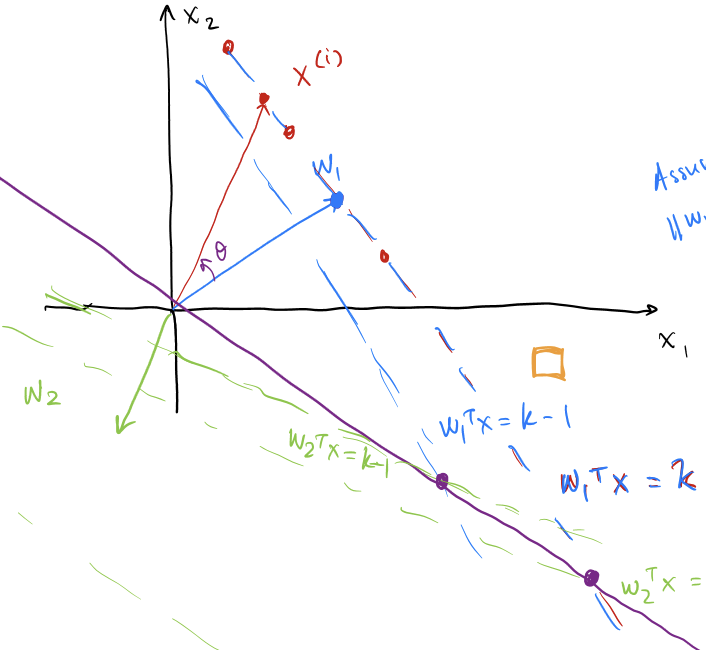
\includegraphics[scale=0.5, trim=0 0 0 0]{lec4_graph.png}
\end{minipage}

We do this through maximum likelihood optimization (maximize the probability of having observed the data).

\tb{Example:} We get data for a coin-flip and we want to choose the probability of heads that maximizes the likelihood of having observed our data. Data = $\{H, T, H, H, T, T, H, T\}$

\tb{Model} $x^{(i)}= \begin{cases} H (1)& w.p \: \theta \\ T (0) & w.p \: 1-\theta \end{cases}$ so we want a $\theta$ with that results in the highest likelihood.

\bit{}
\item \tb{Model 1:} $\theta = 1$ we get $1*0*1*1*0*0*1*0 = 0$
\item \tb{Model 2:} $\theta = 0.75$ we get $(0.75)^4*(0.25)^4 = 0.00124$
\item \tb{Model 3:} $\theta = 0.5$ we get $(0.5)^4*(0.5)^4 = 0.0039$ which is the highest likelihood (\tb{maximum})
\eit{}

We can define a likelihood $\mathcal{L} = \theta^\theta(1-\theta)^4$ and then we can differentiate the $log$ (\tb{because log is monotonically increasing}) of the likelihood with respect to theta and set to $0$ to find $\theta$ maximizing the likelihood of having observed the given data.

In the case of the \tb{softmax} classifier there is not one global optima (maxima in this case) so we cannot just take the derivative but we use gradient descent instead.

\subsection{Chain rule for Probability}
Notations for the class. $Pr(A=a)= p_A(a) = p(a)$ and $Pr(A=a, B=b) = p_{A,B}(a,b)=p(a,b)$

\tb{Chain Rule Example}
$Pr(A=a, B=b) = Pr(A=a)Pr(B=b \: given \: A=a)$ can be written as $p(a,b) = p(a)p(b|a) = p(b)p(a|b)$

We can decompose the probability $p(a,b,c)$ into $p(c)*p(a|c)*p(b|a,c)$ \tb{or} $p(a,c)*p(b|a,c)$ meaning every single outcome goes once in front of the condition bar and every subsequent time they go behind the condition bar.

\tb{example}

$p(b,c|d,e) = \frac{?}{p(d)*p(e|d)}$ if we simplify the bottom into $p(d,e)$ and then move it to the other side and simplify we get $? = p(b,c,d,e)$

\subsection{Softmax Function}
We normalize the scores by turning them into probabilities. The softmax function transforms the class score into a probability via $\text{softmax}_i(\mb{x}) = \frac{e^{a_i(\mb{x})}}{\sum_{j=1}^{c}e^{a_j(\mb{x})}}$ for $a_i(\mb{x}) = \mb{w}_i^T\mb{x}+w_i$ and $c$ being the number of classes, and $a_i(\mb{x}) = \mb{y}_i = \mb{w}_i^T\mb{x}+b_i$ meaing $\mb{a}_i$ is the score if the $i$th class for the image $\mb{x}$ we can also write it as $\mb{a}_i(\mb{x}) = \tilde{\mb{w}}_i^T\mb{x}$ we just removed $b_i$ by concatenating it at the end of each vector in $\mb{W}$ and adding a $1$ to the end of the matrix $\mb{x}$. 

We can see that $0\le \text{softmax}_i(\mb{x})\le 1$ and that the sum of all softmax values is 1.

We use $e$ specifically for connections to information theory when calculating things like the loss which is cross entropy loss, and also since we will be taking the log which will be easy with the $e$.

$\text{softmax}_i(\mb{x}^{(j)}) = Pr(y^{(j)}=i|\mb{x}^{(j)},\theta)$ meaning the softmax of an image, is the probability that the image belongs to the class $i$

\subsection{Softmax Classifier}
Although we know the softmax function, how do we specify the \ti{obejective} or \tb{loss function} to be optimized with respect to $\theta$?

Maybe we should choose the parameters $\theta$ that maximize the likelihood of having seen the data. Assuming the samples, $(\mb{x}^{(1)}, y^{(1)}),...,(\mb{x}^{(m)}, y^{(m)})$ are iid, this corresponds to maximizing:

$p(\mb{x}^{(1)},...,\mb{x}^{(m)},y^{(1)},...,y^{(m)}|\theta) = \prod_{i=1}^mp(\mb{x}^{(i)},y^{(i)}|\theta) = \prod_{i=1}^mp(\mb{x}^{(i)}|\theta)p(y^{(i)}|\mb{x}^{(i)},\theta)$ where $y^{(i)}$ is the class of the image $\mb{x}^{(i)}$ and $\theta = \{\mb{W}, \mb{b}\}$. 

We decompose it in this way because we defined $\text{softmax}_i(\mb{x}^{(j)}) = p(y^{(j)}|\mb{x}^{(j)},\theta)$.

\tb{The assumption that they are iid is necessary for using the product notation (this assumption is broken in video)} or else we would need the first image and class to be behind the condition bar of every subsequent probability.

We want to choose a $\theta$ that makes the data as likely as possible. ${\text{arg max} \atop \theta} \prod_{i=1}^mp(\mb{x}^{(i)}|\theta)p(y^{(i)}|\mb{x}^{(i)},\theta)$ which is equivalent to ${\text{arg max} \atop \theta} \prod_{i=1}^mp(y^{(i)}|\mb{x}^{(i)},\theta)$ because the probability $p(\mb{x}^{(i)}|\theta)$ has no dependence on $\theta$.

Since $log$ is monotonic we can apply it to the probabilities and this turns our product into a sum, so we get ${\text{arg max}\atop \theta}\sum_{i=1}^m log(\text{softmax}_{y^{(i)}}(\mb{x}^{(i)}))$ with the notation $\text{softmax}_{y^{(i)}}(\mb{x}^{(i)})$ we are saying for the $i$th example we have an image and a label $y^{(i)}$ and for that image evaluate the probability that the image belongs to that class.

${\text{arg max}\atop \theta}\sum_{i=1}^m [a_{y^{(i)}}(\mb{x}^{(i)}) - log(\sum_{j=1}^ce^{a_j(x^{(i)})})]$ which we can re-write and add a normalization factor $\frac{1}{m}$ as ${\text{arg min}\atop \theta} \frac{1}{m} \sum_{i=1}^m [ log(\sum_{j=1}^ce^{a_j(x^{(i)})}) - a_{y^{(i)}}(\mb{x}^{(i)})]$ because ${\text{arg max}\atop\theta}f(\theta) = {\text{arg min}\atop\theta}-f(\theta)$

This is loss if called the \tb{cross entropy loss}.

\subsection{Softmax Classifier: Intuition}
When maximizing the softmax the term $a_{y^{(i)}}(\mb{x})$ is made larger and the term $log(\sum_{j=1}^ce^{a_j(x^{(i)})})$ is made smaller. The latter term can be approximated by $\text{max}_j a_j(\mb{x})$.
\bit{}
\item If $a_{y^{(i)}}(\mb{x})$ produces the largest score then the log likelihood is approximately $0$
\item If $a_{j}(\mb{x})$ produces the largest score for $j\ne i$, then $a_{y^{(i)}}(\mb{x})-a_j(\mb{x})$ is negative making the log likelihood negative
\eit{}

So this helps the intuition that when the correct class has the largest score the loss is minimized.

\textbf{Overflow of softmax}
Since a score can be very large causing the value in the numerator of softmax to be even larger it may overflow storage so it is standard practice to normalize by subtracting off the largest score because this has no effect on the resulting softmax.

\section{Lecture 5}

\subsection{Softmax Continued}
Our goal is to optimize and objective function \tb{loss function} $f(x)$ $(\mathcal{L}(\theta)$ (without loss of generality)
\bit{}
\item From basic calculus we know that the derivative of a function tells us the slope of the function at the point.
\item For a small enough $\epsilon$, $f(x+\epsilon)\approx f(x)+\epsilon f'(x)$ telling us how to reduce (or increase) $f(\cdot)$ for small enough steps. This means that we are assuming for a small enough step along the linear approximation we expect the function to be about that value.
\item Recall that when $f'(x)=0$ we are at a critical point can be local/global minimum/maximum or a saddle point.
\eit{}

\tb{Terminology}
\bit{}
\item \tb{Global Minimum:} The point, $x_g$, that achieves the absolute lowest value of $f(x)$
\item \tb{Local Minimum:} The point $x_l$, that is a critical point of $f(x)$ and is lower than neighboring points
\item \tb{Saddle Point:} Critical point of $f(x)$ that are not local minima or maxima, neighboring points are both greater than and less than $f(x)$
\eit{}

Since these loss landscapes are so complicated in general we will be finding local minima but this isn't actually as bad as you may think.

\tb{The Intuition} is that the loss function is a function of our parameters and with lots of parameters $>100000$ the likelihood of being in a local minima (where you cannot search any of the dimensions and get a lower loss) and there being a lower local minima is statistically improbable.

\subsection{Gradient Descent}
Recall the gradient $\Delta_{\mb{x}}f(\mb{x})$ is a vector whose $i$th element is the partial derivative of $f(\mb{x})$ w.r.t $x_i$ the $i$th element of $\mb{x}$. Concretely, for $\mb{x}\in\mathbb{R}^n$

\bit{}
\item The gradient tells us how a small change in $\Delta \mb{x}$ affects $f(x)$ through

$f(\mb{x}+\Delta\mb{x})\approx f(\mb{x})+\Delta\mb{x}^T\nabla_\mb{x}f(\mb{x})$
\item The directional derivative of $f(x)$ in the direction of the unit vector $\mb{u}$ is given by $\mb{u}^T\nabla_\mb{x}f(\mb{x})$
\item The directional derivative tells us the slope of $f$ in the direction of $\mb{u}$ we want a $\mb{u}$ minimizing $f(\mb{x})$.
\item To minimize $f(\mb{x})$ we want to find the direction in which $f(\mb{x})$ decreases the fastest. We do this by finding the direction $\mb{u}$ which minimizes the directional derivative. ${\text{min}\atop\mb{u}, \|\mb{u}\|=1}\mb{u}^T\nabla_\mb{x}f(\mb{x}) = {\text{min}\atop\mb{u}} \|\nabla_\mb{x}f(\mb{x})\|cos(\theta)$ where $\theta$ is the angle between the vectors $\mb{u}$ and $\nabla_\mb{x}f(\mb{x})$
\item The quantity is minimized for $\mb{u}$ pointing in the opposite direction of the gradient, so that $cos(\theta) = -1$
\item Hence we arrive at gradient descent. To update $\mb{x}$ so as to minimize $f(\mb{x})$ we repeatedly calculate $\mb{x} := \mb{x}-\epsilon\nabla_\mb{x}f(\mb{x})$ where $\epsilon$ is typically called the \ti{learning rate}. It can change over iterations and setting it appropriately is an important part of deep learning.
\eit{}

\begin{minipage}{4in}
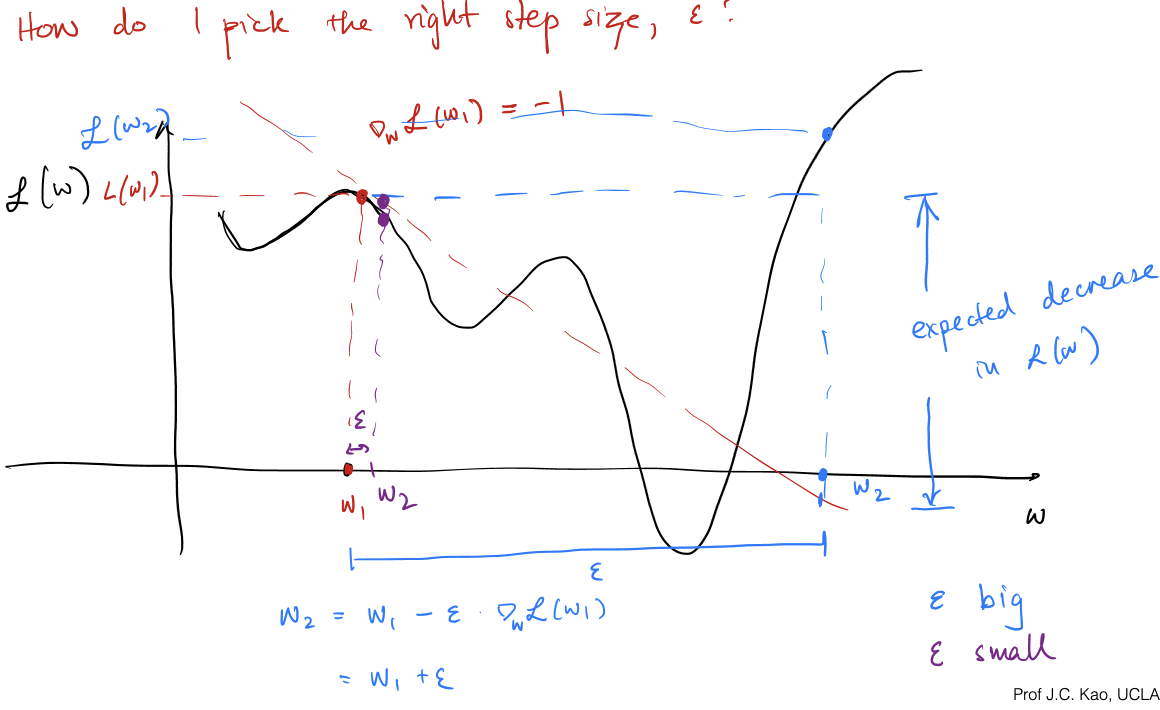
\includegraphics[scale=0.5]{lec5_graph.png}
\end{minipage}
\begin{minipage}{1.2in}
\tb{Interpreting Learning Rates:} Why not just have small learning rate? it takes too long to get to minima. 

You can get a good indication by checking your loss with iterations. If it explodes then learning rate is too high, if it goes slowly it is too low, if it stays constant it is too high. It is perfect when it decreases fast at the beginning and slowly slows down
\end{minipage}

\tb{Why don't we use numerical gradient?} (limit thing)

\bit{}
\item We would have to calculate the gradient for every parameter (bad with lots of parameters)
\item Evaluating $f$ may be expensive (lots of matrix multiplications)
\eit{}

In optimization we differentiate the cost function $f$ w.r.t parameters and the resulting gradient is a function of the training data. So we can think of each data point as providing a noisy estimate of the gradient at that point.

\subsection{Batch vs Minibatch}
It is expensive to calculate the gradient exactly because it requires evaluating the model on all $m$ examples in the data set
\bit{}
\item \tb{Batch Algorithm:} Use all $m$ (e.g. 50000) examples in the training set to calculate a gradient
\item \tb{Minibatch Algorithm:} Approximates the gradient by calculating it using $k$ training examples (usually called \tb{stochastic gradient descent}). We need the class statistics to be as close as the statistics of the full batch as possible because otherwise the model might be trained better for classifying one specific class.
\item \tb{Stochastic Algorithm:} Approximates the gradient by calculating it over some example
\eit{}

% We are optimizing the log likelihood $log(p(\theta))$ but more specifically the expected value (taking into account all examples) $\mathbb{E}_{(\mb{x}^{(i)},y^{(i)} \leftarrow D)}[log(p(\theta))]$ and we want to calculate the gradient of this to update it and continue minimizing. $\nabla_\theta\mathbb{E}_{(\mb{x}^{(i)},y^{(i)} \leftarrow D)}[log(p(\theta))] = \mathbb{E}[\nabla_\theta log(p(\theta))]$ and the expectation is an average over our examples

% $=\frac{1}{m}\sum_{i=1}^m\nabla_\theta log(p(\theta, \mb{x}^{(i)}, y^{(i)}))$ where $m$ is the batch size (e.g. 50000 for full batch)

To get a more robust estimate of the gradient we need to use lots of data samples. 

$J(\theta) = \frac{1}{m}\sum_{i=1}^m log[p_{model}(\mb{x}^{(i)}, y^{(i)} | \theta)$ which is the same as the expected value of the log likelihood. Then taking its gradient we get $\nabla_\theta J(\theta) = \nabla_\theta\frac{1}{m}\sum_{i=1}^m log[p_{model}(\mb{x}^{(i)}, y^{(i)} | \theta) \approx \mathbb{E}[\nabla_\theta log(p_{model}(\mb{x}^{(i)},y^{(i)}|\theta))]$ where $m$ is the batch size. 

As it turns out as well sometimes minibatch is a better approach than the full batch algorithm because having noise leads to more robust answers (generalization benefit).

\subsection{Neural Networks}
Inspired from neurons in neuroscience, neurons are the main signaling units of the nervous system.

\tb{Neurons have four regions:}
\ben{}
\item Cell body (soma) - metabolic center, with nucleus etc
\item Dendrites - tree like structure for receiving \tb{input} signals
\item Axon Hillock - integrative part of the neuron(sums up all inputs from dendrites) and checks if it is bigger than a threshold if so it fires a spike
\item Axon - single, long, tubular structure for sending \tb{output} signals
\item Presynaptic terminals - sites of communication to next neurons
\een{}

The spikes are probabilistic (different every trial even for same stimulus) we think of the spikes as reflecting an underlying rate. This rate is what the neural-networks are \ti{encoding}

\begin{minipage}{2.5in}
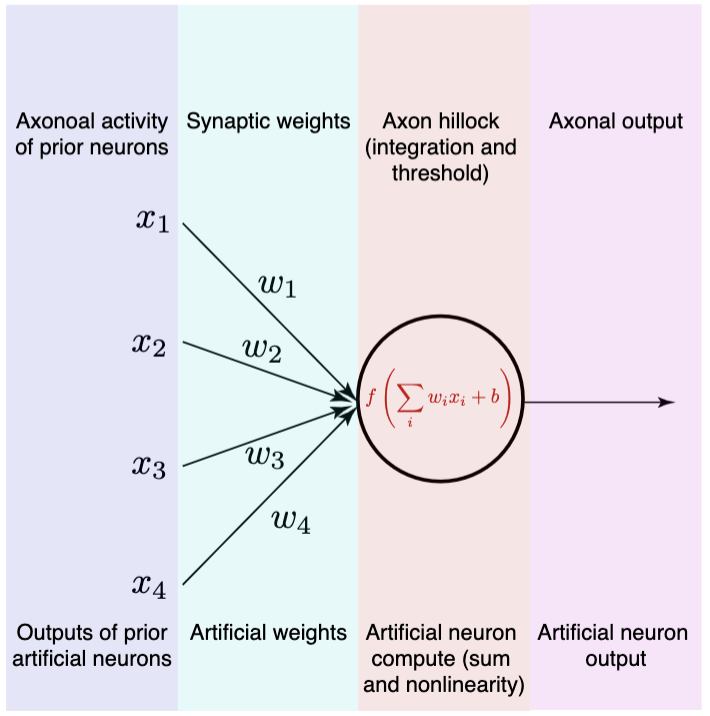
\includegraphics[scale=0.5]{lec5_graph2.png}
\end{minipage}
\begin{minipage}{2.7in}
The $f$ can be the threshold function from neurons but a better activation function is often chosen (can be non-linear)

\tb{Nomenclature}
\bit{}
\item The first layer of a NN is the input layer (represented by $x$)
\item The last layer is the output layer (represented by $z$) think of these as the scores that go to a softmax classifier (often called logits)
\item Intermediate layers are called hidden layers represented with variable $\mb{h}$. For a hidden layer $\mb{h}$ the values are calculated as follows $f(\mb{Wx}+\mb{b})$ where $f$ is the activation function.
\item When we specify that a network has $N$ layers, this does not include the input layer
\eit{}
\end{minipage}

\tb{Intuition behind going to lower dimensional output layer} (4 hidden neurons to 2 output neurons). The number of outputs is the number of classes we have (10 in CIFAR-10) we may want a higher dimensional feature space because it makes separating these 10 classes easier.

\tb{Fully Connected Neural Networks} (sometimes known as Multilayer Perceptron [MLP]) have a connection from every neuron in the previous layer to all neurons in the next layer.

\tb{To calculate the number of learnable parameters} we need the number of weights, $\#\mb{x}\times \#\mb{h}_1 + \#\mb{h}_1\times \#\mb{h}_2+...+ \#\mb{h}_{N-1}\times \#\mb{z}$, plus the number of biases $\#\mb{h}_1+...+\#\mb{h}_{N-1}+\#\mb{z}$

\tb{First layer:} $\mb{h}_1=f(\mb{W}_1\mb{x}+\mb{b}_1)$
\tb{Second layer:} $\mb{h}_2=f(\mb{W}_2\mb{h}_1+\mb{b}_2)$
\tb{(output) layer:} $\mb{z}=\mb{W}_3\mb{h}_2+\mb{b}_3$

\subsection{Activation Function}
What if $f()$  is linear? (e.g. $f(x)=x$. Layer 1: $\mb{h}_1=\mb{W}_1\mb{x}+\mb{b}_1$, Layer 2: $\mb{h}_2=\mb{W}_2\mb{h}_1+\mb{b}_2$ ... Layer N: $\mb{z}=\mb{W}_N\mb{h}_{N-1}+\mb{b}_n$.

Any composition of linear functions can be reduced to a single linear function $\mb{z}=\mb{Wx}+\mb{b}$ where $\mb{W} = \mb{W}_N...\mb{W}_2\mb{W}_1$ and $\mb{b}=\mb{b}_N + \mb{W}_N\mb{b}_{N-1} + ... + \mb{W}_N...\mb{W}_3\mb{b}_2+\mb{W}_N...\mb{W}_2\mb{b}_1$

If $f$ is identity or linear our output $\mb{z}$ is still an affine function of the input $\mb{x}$ and after passing $\mb{z}$ into the softmax we are still just doing linear classification. (nothing more than a linear classifier)

This may be useful in some contexts $\text{dim}(\mb{h}) << \text{dim}(\mb{x})$ (dimensionality reduction), this corresponds to finding a low-rank representation of the inputs.

\tb{Autoencoder} want the loss to be $\mathcal{L}=\|\mb{z}-\mb{x}\|^2$ (we want $\mb{z}$ to look like $\mb{x}$)

\tb{Introducing Nonlinearity} to increase network capacity by adding nonlinear $f(\cdot)$ at the output of each artificial neuron.

Layer 1: $\mb{h}_1=f(\mb{W}_1\mb{x}+\mb{b}_1)$, Layer 2: $\mb{h}_2=f(\mb{W}_2\mb{h}_1+\mb{b}_2)$ ... Layer N: $\mb{z}=\mb{W}_N\mb{h}_{N-1}+\mb{b}_n$.

$f(\cdot)$ is typically called an \ti{activation function} and is applied element-wise to the input.


\section{Lecture 6}
\subsection{What nonlinearity/activation function}
One recurring theme throughout neural network design is that the gradient of the cost function must be large and predictable enough to serve as a good guide for the learning algorithm.

\tb{Sigmoid Unit:}

$\sigma(x) = \frac{1}{1+exp(-x)}$ where $\frac{\partial \sigma (x)}{\partial (x)} = \sigma(x)(1-\sigma(x))$

Our cost/loss function $\mathcal{L}(\mb{w})$ is a function of our weights $\mb{w}$ in this example we'll have $\mb{w}$ as a vector not matrix $\sigma(\mb{w}) = \sigma(\mb{w}^T\mb{x}+\mb{b})$ and when we are doing gradient descent we update our weights $\mb{w}$ as follows $\mb{w}\leftarrow \mb{w}-\epsilon\frac{\partial \mathcal{L}}{\partial\mb{w}}$ and from the quote above we want $\frac{\partial \mathcal{L}}{\partial\mb{w}}$ to be large.

By the chain rule $\frac{\partial \mathcal{L}}{\partial\mb{w}} = \frac{\partial \sigma(\mb{w})}{\partial\mb{w}} \frac{\partial\mathcal{L}}{\partial\sigma(\mb{w})}$

The input to our sigmoid is $\mb{w}^T\mb{x}+b_1$ there are locations in the sigmoid where the input (if it's too big or too small) then our $\frac{\partial \sigma(\mb{w})}{\partial\mb{w}}$ will be very small making the overall gradient very small meaning there will be little to no learning.

\bit{}
\item[$+$] around $x=0$ the unit behaves linearly, and it is differentiable everywhere
\item[$-$] At extremes the unit \ti{saturates} and has zero gradient resulting in no learning
\item[$-$] The sigmoid unit is non-negative. SGD with the sigmoid unit will zig-zag (in practice not too much concern) e.g. if $f(\mb{w})=\sigma(\mb{w}^T\mb{h}_1+b)$ and $z=\mb{w}^T\mb{h}_1+b$ we can say $\frac{\partial f(\mb{w})}{\partial \mb{w}} = \frac{\partial z}{\partial\mb{w}}\frac{\partial f(\mb{w})}{\partial z} = \sigma(z)(1-\sigma(z))\mb{h}_1$ where the entire gradient $\frac{\partial f(\mb{w})}{\partial\mb{w}}$ is $\ge 0$. Remember we calculate the gradient descent steps as $\frac{\partial \mathcal{L}}{\partial \mb{w}} = \frac{\partial f(\mb{w})}{\partial\mb{w}} \frac{\partial \mathcal{L}}{\partial f(\mb{w})}$ where the second term is a scalar with values $\ge 0$ or $\le 0$ meaning the steps made by gradient descent can either be all weights in the negative direction or all weights in the positive direction. So if the minima is in a place where some weights are negative and some are positive it will have to zig-zag.
\eit{}

\tb{Hyperbolic Tangent}, $\text{tanh}(x)=2\sigma(2x)-1$, the hyperbolic tangent is a zero-centered sigmoid-looking activation. And $\frac{\partial \text{tanh}(x)}{\partial x} = 1-\text{tanh}^2(x)$

\bit{}
\item[$+$] Around $x=0$ unit behaves linearly, differentiable everywhere, and zero-centered (no zig-zag)
\item[$-$] Like the sigmoid unit, when a unit saturates (values grow larger or smaller), no additional learning occurs (gradients 0)
\eit{}

\tb{Rectified Linear Unit}, $\text{ReLU}(x) = max(0,x)$ and $\frac{\partial\text{ReLU}(x)}{\partial x} = \begin{cases} 1 & x>0\\ 0 & x < 0 \end{cases}$ this function is not differentiable at $x=0$ However we can define its subgradient to be between [0,1] at $x=0$.

\tb{When x is positive the gradient is 1}

\bit{}
\item[$+$] In practice, learning with ReLU converges faster than sigmoid and tanh (6x faster)
\item[$+$] When a unit is active, it behaves as a linear unit
\item[$+$] The derivative at all points (besides 0) is 0 or 1, no saturation if $x>0$
\item[$-$] $\text{ReLU}(x)$ is like sigmoid it zig-zags, and not differentiable at $x=0$ not big issue
\item[$-$] Learning doesn't happen for examples with zero activation (fixed with leaky ReLU or maxout)
\eit{}

\tb{Softplus unit}, $\zeta(x) = log(1+exp(x))$ with $\frac{\partial\zeta(x)}{\partial x} = \sigma(x)$ it resembles ReLU but it is differentiable everywhere so maybe it performs better, but empirically it performs worse.

\tb{Leaky ReLU/PReLU (learnable alpha)}, $f(x) = max(\alpha x, x)$ where $\alpha = 0.01$ and can be a hyperparameter. The leaky ReLU avoids dead units when $x<0$ allowing learning to continue.

\tb{Exponential Linear Unit ELU}, $f(x) = max(\alpha(exp(x)-1),x)$ this is very similar to Leaky ReLU except it requires more computation because of $e^x$

\tb{Swish}, $\text{swish}(z) = x\sigma(\beta x) = \frac{x}{1+e^{-\beta x}}$ again similar to ReLU.

\tb{The output activation interacts with the cost function}

For example let's say our output is a scalar $z$ and if we have a large positive $z$ we predict class 1, and when we have a large negative $z$ we predict class 0. $\sigma(z) = Pr\{x^{(i)} \text{belongs to class} 1\}$ the softmax function is the multiclass generalization of this sigmoid for binary classification.

Is it better to use \tb{MSE} or \tb{CE} as the cost function where $\text{MSE} = \frac{1}{2}\sum_{i=1}^n(y^{(i)}-\sigma(z^{(i)}))^2$ and $\text{CE} = -\sum_{i=1}^n[y^{(i)}log \sigma(z^{(i)})+(1-y^{(i)})log(1-\sigma(z^{(i)}))]$

\tb{MSE} as a loss function is a very poor choice because when we're far away from the answer (large negatives/positives) changing our input to the activation will not change the loss at all which is unhelpful. If we start off with a bad answer we will never change it to become a better value.

Whenever you have an output that is sigmoid or softmax we never want to use \tb{MSE} loss we always want to use some loss like \tb{CE}

\subsection{Backpropogation}
The neural network will have multiple layers with weights and biases for these layers $\mb{W},\mb{b}$ and activation functions $f$ in between the layers. The output of the neural network is then passed to softmax where we get our final loss $\mathcal{L}$

Our learning rule is \tb{SGD} so $\theta\leftarrow \theta-\epsilon\frac{\partial \mathcal{L}}{\partial \theta}$ but we don't know this gradient which are $\frac{\partial \mathcal{L}}{\partial \mb{W}_i}$. The algorithm to calculate these gradients is called backpropogation. All it is is a fancy name for the chain rule of calculus (applies the chain rule in an operationalized fashion)

\tb{Forward propogation/forward pass:} start at input and do neural network operations to calculate $\mb{z}$ and then $\mathcal{L}$

\tb{Backpropogation/Backward pass:} start with the derivative $\frac{\partial\mathcal{L}}{\partial\mb{z}}$ (gradient of the loss with respect to the softmax scores) then running backwords through the network to compute $\frac{\partial \mathcal{L}}{\partial \mb{w}_3}$ then $\frac{\partial \mathcal{L}}{\partial \mb{w}_2}$, $\frac{\partial \mathcal{L}}{\partial \mb{w}_1}$

\tb{Why do we need backpropogation?}

\bit{}
\item Backpropogation is computationally efficient because we find most of the terms needed in backprop can be cached from forward pass
\item Informally sometimes taking analytical multivariate gradients can be challenging. Backprop breaks these down into easier steps
\item It is not the learning algorithm it is the method for computing gradients
\item It is not specific to multi-layer NNs but a general way to compute derivatives
\eit{}

The \tb{upstream gradient} is the derivative of the loss function with respect to the last wire in the network. (typically gradient of the loss with respect to the softmax classifier).

\tb{Basic step w/ chain rule}, if we are looking to find $\frac{\partial \mathcal{L}}{\partial z}$ we know by the chain rule that it is $\frac{\partial f}{\partial z} \frac{\partial \mathcal{L}}{\partial f}$ which means the local gradient times the upstream gradient.

The basic intuition of backpropogation is that we break up the calculation of the gradient into \tb{small and simple steps}. Each of these nodes in the graph is a straightforward gradient calculation where we multiply an \tb{input} (upstream derivative/gradient) with a \tb{local derivative/gradient} (chain rule)

\subsection{Backpropogation Rules}
Rules we can derive from backpropogation steps on simple examples.
\bit{}
\item \tb{Addition:} Just pass the upstream gradient through
\item \tb{Multiplication:} Take the upstream gradient and multiply by the value on the other wire
\item \tb{Max:} Take the upstream gradient and multiply it by the indicator function if $x>y$ where $x$ is the wire we are finding the gradient for. e.g. $\mathbb{I}(x>y) \frac{\partial \mathcal{L}}{\partial f}$
\item \tb{Inv:} Upstream gradient times $-\frac{1}{x^2}$ where $x$ is the value on the wire
\item \tb{Exp:} If we have a wire $b$ which is the output of a $exp$ gate with $c$ as input e.g. $b=e^{c}$ the local gradient $\frac{\partial b}{\partial c} = e^c$ so we take that and multiply by the upstream
\item \tb{Log (natural):} Upstream gradient times $\frac{1}{x}$
\item \tb{Transpose:} Transpose the upstream gradient
\eit{}

The local gradient of a node (function) is calculated by taking the derivative of it with respect to its inputs.

\tb{What happens when two gradient paths converge?} Two wires going to the same node e.g. we have a node $h$ with two wires coming off of it $q_1=h(x)$ and $q_2=h(x)$ (because the input to the $h$ node is $x$. What is our gradient $\frac{\partial \mathcal{L}}{\partial x}$? By law of total derivative the gradient $=\sum_{i=1}^n \frac{\partial q_i}{\partial x} \frac{\partial \mathcal{L}}{\partial q_i}$

\section{Lecture 7}
To do multivariate backpropogation, we need a multivariate chain rule. (Matrices and vectors)

\subsection{Derivative of a Vector w.r.t a Vector}
Let $\mb{y} \in \re^m$, what dimensionality should the derivative of $\mb{y}$ with respect to $\mb{x}$ be?

\bit{}
\item e.g. to see how $\Delta\mb{x}$ modifies $y_i$, we would calculate $\Delta y_i = (\nabla_\mb{x}y_i)^T\Delta\mb{x}$
\item This suggests that the derivative ought to be an $n\times m$ matrix, denoted $\mb{J} = \bms (\nabla_\mb{x}y_1)^T \\ (\nabla_\mb{x}y_2)^T \\ ... \\ (\nabla_\mb{x}y_n)^T\bme$ where $(\nabla_\mb{x}y_i)^T = \bms \frac{\partial y_i}{\partial x_1} & \frac{\partial y_i}{\partial x_2} & ... & \frac{\partial y_i}{\partial x_m}\bme$ This matrix would tell us how a small change in $\Delta\mb{x}$ results in a small change in $\Delta\mb{y}$ according to the formula $\Delta\mb{y} \approx \mb{J}\Delta\mb{x}$
\item The matrix $\mb{J}$ is called the \tb{Jacobian} $\in \re^{n\times m}$ and it tells how wiggling a vector $\Delta\mb{x}$ affects another vector $\Delta\mb{y}$
\eit{}

\tb{In the denominator layout definition, the denominator vector changes in a column} e.g. $\derv{\mb{y}}{\mb{x}} = \bms \derv{\mb{y}_1}{\mb{x}} & \derv{\mb{y}_2}{\mb{x}} & ... & \derv{\mb{y}_n}{\mb{x}}\bme$ and each element $\derv{\mb{y}_i}{x} = \bms \derv{\mb{y}_i}{\mb{x}_1} \\ \derv{\mb{y}_i}{\mb{x}_2} \\ ... \\ \derv{\mb{y}_i}{\mb{x}_m} \bme$

\tb{Think about it as the dimension of the vector in the denominator is the first dimension of the resulting matrix}

Hence the notation we use for the \tb{Jacobian} in denominator form would be $(\grad{\mb{x}}{\mb{y}})^T$ ($y$s change in column $x$s change in row)

\tb{Example:} $\grad{\mb{x}}{\mb{y}} = \mb{W}^T$ when $\mb{y} = \mb{Wx}$ because $\mb{x}\in \re^n$, $\mb{y}\in\re^h$ and $\grad{\mb{x}}{\mb{y}}\in\re^{n\times h}$

\tb{Hessian}

The multivariate generalization of a second derivative. (the gradient of the gradient $\grad{\mb{x}}{(\grad{\mb{x}}{f(\mb{x})})}$

\subsection{Multivariate (Vector) Chain Rule}
\tb{From the scalar chain rule} we know if $y=f(x)$ and $z=g(y)$, then $\derv{z}{x}=\derv{y}{x}\derv{z}{y}$ (intuitavely how wiggling $x$ wiggles $z$ by first seeing how it wiggles $y$ then seeing how $y$ wiggles $z$)

\tb{For vectors}, we have $\mb{x} \in \re^m$, $\mb{y} \in \re^n$ and $\mb{z} \in \re^p$ with $\mb{y}=f(\mb{x})$ and $\mb{z}=g(\mb{y})$

\bit{}
\item $\Delta\mb{x}\rightarrow\Delta\mb{z}$ (how wiggling $\mb{x}$ wiggles $\mb{z}$)
$\Delta\mb{z} \approx (\derv{\mb{z}}{\mb{x}})^T\Delta\mb{x} \rightarrow (p)\approx(p\times m)(m)$
\item $\Delta\mb{x}\rightarrow\Delta\mb{y}\rightarrow\Delta\mb{z}$ (how wiggling $\mb{x}$ wiggles $\mb{y}$ wiggles $\mb{z}$)
$\Delta\mb{y} \approx (\derv{\mb{y}}{\mb{x}})^T\Delta\mb{x} \rightarrow (n)\approx(n\times m)(m)$ and $\Delta\mb{z} \approx (\derv{\mb{z}}{\mb{y}})^T\Delta\mb{y} \rightarrow (p)\approx(p\times n)(n) = (\derv{\mb{z}}{\mb{y}})^T(\derv{\mb{y}}{\mb{x}})^T\Delta\mb{x}$
\eit{}

\tb{Tensor Derivatives}

$\mb{y}=\mb{Wx}$ in a NN this corresponds to $\mb{h_2}=f(\mb{W_2h_1})$ in this example $\mb{y}\in\re^m$, $\mb{x}\in\re^n$ and $\mb{W}\in\re^{m\times n}$

$\derv{\mb{y}}{\mb{W}}\in\re^{m\times n\times m}$ remember $\derv{\mb{y}_1}{\mb{W}}\in\re^{m\times n}$ and we will just stack $\forall_{i=1}^m \derv{\mb{y}_i}{\mb{W}}$ matrices resulting in a tensor $\in\re^{m\times n \times m}$

\tb{Example:} $\derv{\mb{z}}{\mb{W}}\in\re^{m\times n\times m}$ where $\mb{z}\in\re^m$, $\mb{x}\in\re^n$ and $\mb{z}=\mb{y}-\mb{Wx}$

$\derv{\mb{z}_k}{\mb{W}} \in\re^{m\times n}$ (there will be $m$ of these $k=\{1,...,m\}$ it will have $0$s in every single row except the $k$th row where the row will be $\bms -\mb{x}_1 & -\mb{x}_2 & ... & -\mb{x}_n\bme$


\tb{A few notes on tensor derivatives}

\bit{}
\item In general, the simpler rule can be inferred via pattern intuition / looking at the dimensionality of the matrices, and these tensor derivatives need not be explicitly derived
\item Actually calculating them and storing them is usually not a good idea for memory and computation reasons
\item If we know the end result is a simple outer product of two vectors, we need not even calculate an additional derivative in this step of backpropogation (assuming inputs were cached)
\eit{}

\tb{Intuition}, since we know $\grad{\mb{x}}{\mb{Wx}} = \mb{W}^T$ then $\grad{\mb{W}}{\mb{Wx}}$ ought to look like $\mb{x}^T$. We know that $\derv{\epsilon}{\mb{z}}\in\re^m$ and $\derv{\epsilon}{\mb{W}}\in\re^{m\times n}$. By the chain rule $\derv{\epsilon}{\mb{W}} = \derv{\mb{z}}{\mb{W}}\derv{\epsilon}{\mb{z}}$ and because $\derv{\epsilon}{\mb{W}}\in\re^{m\times n}$ and $\derv{\epsilon}{\mb{z}}\in\re^{m\times 1}$ if we said that instead of $\derv{\mb{z}}{\mb{W}}$ being a tensor it looked like $\mb{x}^T\in\re^{1\times n}$ and we multiplied it on the other side for an outer product we would get the correct answer, meaning $\derv{\epsilon}{\mb{W}} = \derv{\epsilon}{\mb{z}}\mb{x}^T$

\tb{THIS TRICK WORKS WITH MATRICES TIMES MATRICES TOO}

\tb{Example with backprop:}
$\mb{y}=\mb{Wx}$ then $\derv{\mal}{\mb{x}} = \mb{W}^T\derv{\mal}{\mb{y}}$ and $\derv{\mal}{\mb{W}} = \derv{\mal}{\mb{y}}\mb{x}^T$

Any operation in the computational graph that is applied element wise (like ReLU) will result in a hadamard product. e.g. If we have an input to a ReLU $\mb{x}$ and its outputs $\mb{h}_2$ (both vectors) the backprop $\derv{\mal}{\mb{x}} = \mathbb{I}\{\mb{x}>0\}\odot \derv{\mal}{\mb{h}_2}$

\subsection{Initializations}
The initializations of weights in biases for each neural network layer have an impact on the model. If for example we set them all as \tb{small random weights} $w_{i,j} \leftarrow N(0, 0.01)$ where $N(0,0.01)$ means a normal distribution with $0$ mean and $0.01$ variance. \tb{Xavier Initialization} is $w_{i,j}\leftarrow N(0,\frac{1}{n})$ where $n$ is the number of neurons in the prior layer. 

\tb{It is bad for learning if the output activations are close to zero} because $\derv{\mal}{\mb{W}} = 0$ so no learning occurs.

\section{Lecture 8}

\subsection{Initializations Continued}
\tb{Large random weight initialization:} $w_{i,j}\leftarrow N(0,1)$ our activations will explode with the means and standard deviations of the activations being very high at later hidden layers. This is bad because in gradient descent we will be taking large gradient steps and our gradient will not converge.

\tb{If not small and not large initialization, then what?}

\subsection{Xavier initialization}
We want the variances of the activations in layer 1 to equal the variances of the activations in layer 2 ... to the last layer. (keep the variance of the units similar between each layer).

For simplicity, we assume the input has equal variance across all dimensions. Then, each unit in each layer ought to have the same statistics. $h_i$ denotes a unit in the $i$th layer, but the variances ought to be the same for all units in this layer.

\tb{Concretely} $\text{var}(h_i)=\text{var}(h_j)$ and $\text{var}(\grad{h_i}{\mb{J}})=\text{var}(\grad{h_j}{\mb{J}})$. We are going to assume that each artificial neuron in one layer has the same statistics as eachother (same expected value and variance etc). How do we set the weights initially so that the variance of the neurons in every layer are equal.

\tb{Assuming} the units are linear, then $h_i = \sum_{j=1}^{n_{in}}w_{i,j}h_{i-1,j}$ where each layer has $n_{in}$ neurons. Further if $w_{i,j}$ and $h_{i-1}$ are independent, and all the units in the $(i-1)$th layer have the same statistics, using the fact $\vt{var}(wh)=\ex^2(w)\vt{var}(h)+\ex^2(h)\vt{var}(w)+\vt{var}(w)\vt{var}(h)$ which is the same as $= \vt{var}(w)\vt{var}(h)$ if $\ex(w)=\ex(h)=0$ then $\vt{var}(h_i)=\vt{var}(h_{i-1})\cdot\sum_{j=1}^{n_{in}}\vt{var}(w_{i,j})$ so we want this \tb{sum} to be $1$

Because we are assuming the statistics are shared between all activations then $n_{in}\times \vt{var}(w) = 1$ solving for variance we get $\vt{var}(w) = \frac{1}{n_{in}}$ \tb{Which is what we will initialize the variance of our weights to be so our activations don't explode or become 0}

Since we also wanted the gradients to have similar variances we get for each connection $j$ in layer $i$ $\vt{var}(w_{i,j}) = \frac{1}{n_{out}}$ so we incorporate both of these in the Xavier initialization by setting the weight distribution to $N(0,\frac{2}{n_{in}+n_{out}})$ \tb{but oftentimes the nout is left out}

\tb{Important Note:} If we use this Xavier initialization $\frac{1}{n_{in}}$ with ReLU lots of the units will go to 0 instead. If we assume that ReLU will kill off $50\%$ of our units so we should increase the variance by a factor of 2, motivating $\frac{2}{n_{in}}$. Eventually it is suggested to use a uniform distribution $U(-\frac{\sqrt{6}}{n_{in}+n_{out}}, \frac{\sqrt{6}}{n_{in}+n_{out}})$

\subsection{Batch Normalization}
Will help neural network be far less sensitive to hyperparameter settings and initializations

\tb{Motivated through internal covariate shift, but also works by making the loss surface smoother}

Take a neural network where we have multiple layers, say we are trying to update the weights of the third layer $w_3$ we do this through the update step $w_3\leftarrow w_3-\epsilon\grad{\mal}{w_3}$ the problem is we are only updating it by looking at how wiggling $w_3$ will change the loss but the loss can also be changed by other things not just $w_3$ and at every gradient descent step we are updating all weights meaning the gradients which we had calculated based on the output of a previous layer are now stale because we updated the previous layer with gradient descent as well. (this is dangerous because we update the weights in parallel)

This can be avoided by having some vector $\tilde{w}$ which has all weights in it and we then take $\grad{\mal}{\tilde{w}}$ because we will be seeing how wiggling all weights will effect the loss.

\tb{The idea of batch normalization} is that we know when $w_3$ is changing it expected $h_2$ to have the statistics from the last training batch (not the statistics after update). We mitigate this by normalizing all the statistics of the hidden unit activation to be $0$ mean unit variance.

$h_i = \vt{relu}(x_i)$ where $x_i$ is the input (usually $W_ih_{i-1}$) then we want to normalize $\ex[x_i] = 0$ and $\vt{var}[x_i] = 1$

So our NN will look like \tb{affine}$\rightarrow$\tb{BN}$\rightarrow$\tb{ReLU}$\rightarrow$\tb{affine}... so we apply the batch norm before the ReLU

When we have \tb{batch normalization} we don't need \tb{Xavier initialization} (because of BN needing $\vt{var}[x_i] = 1$) but it likely still helps

\tb{Batch-Norm can be thought of as z-scoring}

For a batch of $m$ training examples of activations (before the ReLU) we can compute the mean. $\mu_i = \frac{1}{m}\sum_{j=1}^mx_i^{(j)}$ and the standard deviation $\sigma_i^2=\frac{1}{m}\sum_{j=1}^m(x_i^{(j)}\mu_i)^2$ after computing these we make it $0$ mean by subtracting the mean and unit variance by dividing the stdev (plus some small $\epsilon$ to ensure no divide by $0$)

$\hat{x}_i=\frac{x_i-\mu_i}{\sqrt{\sigma_i^2+\epsilon}}$, where $\hat{x}_i$ is our normalized activation. The output of the batch norm layer will be a $y_i=\gamma_i\hat{x}_i+\beta_i$ with $\gamma_i$ and $\beta_i$ being learnable parameters allowing $\ex[y_i]=\beta_i$ and $\vt{var}[y_i]=\gamma_i^2$. (shift and scale parameters)

\tb{Why did we go through the trouble of getting 0 mean unit variance if we can just change it with parameters?} If we restrict it that much we may overly constrain the network which may not allow the lowest loss.

\tb{Layer Normalization} is the same as batch-normalization but taking $m$ as the number of activations in the layer not just some batch.

\tb{Group Normalization} is normalizing over groups in the layer so if the first 10 activations are a group we could normalize over those then the next 10 etc.

\tb{Back propogation for batch normalization} (for one unit $i$ and one example $j$) there are $m$ total examples

The batch normalization layer is typically placed right before the nonlinear activation. Hence, a layer of a neural network may look like $\mb{h}_i=f(\vt{batch-norm}(\mb{W}_i\mb{h}_{i-1}+\mb{b}_i))$

Empirically, batch normalization allows higher learning rates to be used (with no batch-norm you typically need lower learning rates) this is because \tb{batch-norm} is making the loss surface smoother so the likelihood if computing a large gradient is rarer so you can have the learning rate set higher.

\section{Lecture 9}
\subsection{Regularizations}
Regularizations are used to improve model generalization. \tb{[Regularization is] any modification we make to a learning algorithm that is intended to reduce its generalization error but not its training error}

\bit{}
\item Tends to increase the estimator bias while reducing the estimator variance
\item Can be seen as a way of preventing overfitting
\item Common problem is picking the model size and complexity, it may be fine to choose a large model with good regularization
\eit{}

\tb{Early Stopping}

Constantly evaluate the training and validation loss on each iteration and return the model with the lowest validation error. 

\subsection{Norm Penalties}

A common and simple type of regularization is to modify the cost function with a parameter norm penalty. This penalty is typically denoted as $\Omega(\theta)$ and results in a new cost function of the form $\mal(\theta;\mb{X},\mb{y})+\alpha\Omega(\theta)$ where $\alpha\ge 0$ and it dictates how much you care about the parameter norm penalty over the original loss (hyperparameter, can strongly affect generalization).

\tb{$L^2$ regularization}

Penalize the size of weights, also called \ti{ridge regression} this promotes models with parameters that are closer to $0$ (simpler). $\Omega(\theta)=\frac{1}{2}\mb{w}^T\mb{w} = \frac{1}{2}\|\mb{w}\|^2$. Intuitively, to prevent $\Omega(\theta)$ from getting large $L^2$ regularization will cause weights $\mb{w}$ to have small norm.

The new cost function is $\tilde{\mal}(\mb{w};\mb{X},\mb{y})=\mal+\frac{\alpha}{2}\mb{w}^T\mb{w}$ with the corresponding gradient $\grad{\mb{w}}{\tilde{\mal}}=\alpha\mb{w}+\grad{\mb{w}}{\mal}$ so our update step now becomes $\mb{w}\leftarrow(1-\epsilon\alpha)\mb{w}-\epsilon\grad{\mb{w}}{\mal}$ formalizing the shrinking of weights (weight decay)

\tb{Why we want smaller weights example:} Say we want $y=1$ with $x_1 = 0.1$ and $x_2 = 0.01$ to make $1$ we can do $100x_1-900x_2$ but now if we have small deviations in the inputs say $x_1=0.11$ our prediction would now be $2$ \tb{when we have large weights we're more sensitive to fluctuations in the inputs}

\tb{Extensions of $L^2$ regularization}

Instead of a soft constraint that $\mb{w}$ be small, one may have prior knowledge that $\mb{w}$ is close to some value $\mb{b}$. Then the regularizer may take the form: $\Omega(\theta)=\|\mb{w}-\mb{b}\|_2^2$ or if we want $\mb{w}^{(1)}$ and $\mb{w}^{(2)}$ to be close we can have $\Omega(\theta)=\|\mb{w}^{(1)}-\mb{w}^{(2)}\|_2^2$

\tb{$L^1$ Regularization} instead of penalizing the 2-norm we penalize the 1-norm

$\Omega(\theta)=\|\mb{w}\|_1 = \sum_i|w_i|$ Intuitively this penalty also causes the weights to be small. However, because the subgradient of $\|\mb{w}\|_1$ is $\text{sign}(\mb{w})$ the gradient is the same regardless of the size of $\mb{w}$ (think of the graph of the absolute value). The gradients of the 1-norm are always the same. Empirically if we penalize the weights with the 1-norm the weights will go to $0$

\bit{}
\item This may be useful for feature selection, because features with $0$ weights are discarded (because they weren't useful for predicting the output)
\eit{}

\tb{Pruning the network} do an $L^1$ regularization and remove the features with weights $0$ (this leads to smaller models [more memory saving])

\tb{Sparse Representations} instead of having sparse parameters (e.g. elements of $\mb{w}$ being sparse) we may want to have sparse representations. Imagine a hidden layer of activity $\mb{h}^{(i)}$ to achieve this we may set $\Omega(\mb{h}^{(i)})=\|\mb{h}^{(i)}\|_1$

\subsection{Dataset Augmentation}
We can flip the image, crop it, adjust the brightness, lens correction, rotate. By doing these dataset augmentations we increase the size of our training data and increase the robustness of the classification for those images.

\tb{Label Smoothing} add noise to network by saying our labels are noisy. Instead of having a \ti{one hot} representation of the label for a given image (a vector with all $0$s for each class the image is not and a single $1$ for the index of class the image is part of) we can have label smoothing where each label index has a probability (so instead of a single 1 we have something like $0.9$ for the correct class and distribute the remaining $0.1$ across all other class indexes).

\tb{Cross Entropy Loss for one hot} $\mal^{(i)}=\sum_{c=1}^C-y_clog(p_c)$ where $y_c$ is either $0$ or $1$ (if correct class), and $p_c$ is the probability of the model for the class.

\tb{Cross Entropy Loss for label smoothing} $\mal^{(i)}=-y_c(1-\alpha)*log(p_c)+\frac{\alpha}{C-1}$ where $y_c\in\{0,1\}$, $\alpha = 0.1$ (hyperparameter) (probability for the incorrect class), $C$ is the number of classes and $-y_c(1-\alpha)*log(p_c)$ is the negative log likelihood for the correct class. (the $\frac{\alpha}{C-1}$ should be summed for all incorrect classes)

\tb{Multitask Learning}
If we have one task like image-net classification it may lead to features specific to the classification problem but in general is looking at the image and determining what it is and a lot of the features used for this may be used for other classification tasks. (example tasks below)

\bit{}
\item \tb{Semantic Decoding:} Labeling the class of every pixel
\item \tb{Instance Decoding:} Labeling all the instance of one class
\item \tb{Depth Decoding:} Seeing how far something is in a given image
\eit{}

We can say that the output of a neural network must use these tasks. For each of these tasks (decodings) we have a loss and the multi-task loss is a sum or weighted sum of these. When we compute the gradients we back propogate through the entire network, now each of these tasks share the same features from the NN (upstream) this has the regularizing effect of helping the features be more general.

\tb{Transfer Learning} (good to prevent overfitting for tasks with little data)

The idea is that if tasks are similar enough, then the features at later layers of the network ought to be good features for the new task. If little training data is available but the tasks are similar you just train a new linear layer at the output of the pre-trained network. Even if more data is available for the task it may still be good to use transfer learning.

We freeze the trained network from the similar task and just train the new linear layer at the output with the limited data.

\subsection{Ensembling}
Approach is to train multiple different models and average their results together at test time. (because the models might make independent errors)
\tb{This almost always increases performance by substantial amounts}

\tb{Intuition} is that if they are independent models they will make independent errors

With $k$ independent models, the average model error will decrease by a factor of $\frac{1}{k}$. Denoting $\epsilon_i$ to be the error of model $i$ on an example and assuming $\ex\epsilon_i=0$ means the statistics of the error is the same across all models.

$\ex[(\frac{1}{k}\sum_{i=1}^k\epsilon_i)^2] = \frac{1}{k}\ex\epsilon_i^2$ (if the models make independent errors)

$\frac{1}{k}\ex\epsilon_i^2+\frac{k-1}{k}\ex[\epsilon_i\epsilon_j]$ (if the models are not independent) worst case they make the same mistakes $\epsilon_i= \epsilon_j$

\tb{Bagging} (bootstrap aggregating)

The way we make $k$ models to average is by making $k$ datasets where we draw $N$ examples from the training set with replacement, we do this for $k$ datasets.

\bit{}
\item Construct $k$ datasets using the bootstrap (Data size $N$ and draw with replacement to get $N$ samples, do this $k$ times e.g. $k=2$ $N=\{1,2,3,4\}$ we could have dataset 1 $=\{1,2,1,3\}$ and dataset 2 $=\{4,3,2,3\}$)
\item Train $k$ models on these $k$ datasets
\eit{}
In practice, neural networks reach a wide variety of solutions with different initializations, hyperparameters etc meaning even if trained from same dataset they tend to produce partially independent errors. ($k$ models with different inits where we train on the same dataset)

\tb{Model averaging is very expensive}

\subsection{Dropout}
The way we get the benefit of ensembling in neural networks. Dropout is a computationally inexpensive yet effective method for generalization. It can be viewed as \tb{approximating the bagging procedure} for exponentially many models, while only optimizing a single set of parameters.

\bit{}
\item On a given training iteration sample a binary mask (each element $\in\{0,1\}$) where $1$ occurs w.p $p$ and $0$ w.p $1-p$
\item One hyperparameter per layer $p$ which is the probability of keeping a neuron in a layer, typical values $p=0.8$ for inputs and $p=0.5$ for hidden units
\item Apply the mask to all units (hadamard product) then perform forward and backward pass and parameter update
\item In \ti{prediction}, multiply each hidden unit by the parameter of its Bernboulli mask, $p$
\eit{}

If we have a NN with $N$ units there are $2^N$ possible masks, in every epoch we change the mask we use for dropout.

\tb{What about test time?} e.g. Training iteration 1 $M=[1,0,1,0]\Rightarrow h_{out}=\text{relu}(w_1h_1+w_3h_3)$ Training iteration 1 $M=[0,1,0,1]\Rightarrow h_{out}=\text{relu}(w_2h_2+w_4h_4)$

Naively if we said $h_{out}=\text{relu}(w_1h_1+w_2h_2+w_3h_3+w_4h_4)$ but the statistics of this $h_{out}$ don't match the statistics of the training. To make them correct we scale by $p$ e.g. $h_{out}=\text{relu}(w_1h_1+w_2h_2+w_3h_3+w_4h_4)*p$ this is called the \tb{weight scaling inference rule}

\subsection{Inverted Dropout}
With regular \tb{Dropout} we need our $p$ in testing but we don't want that. Instead we use \tb{Inverted Dropout}. When we generate the mask it's no longer just $1$s and $0$s but $1$s and $0$s divided by $p$ (this can be done either to the mask or the activations). This will scale the activations in training so that in test time we don't have to multiply by $p$.

\tb{How is this a good idea?}
\ben{}
\item Dropout approximates bagging since each mask is basically a different model
\item Think of the dropout as regularizing each hidden unit to work well in different contexts (masks)
\item Dropout may cause units to encode redundant features (multiple neurons encode necessary features for classification)
\een{}

\section{Lecture 10}

\subsection{Optimization for Neural Networks}
Can we improve the SGD algorithm?

\tb{Vanilla GD:} the gradient descent step is $\theta\leftarrow\theta-\epsilon\grad{\theta}{\mal(\theta)}$ where $\mal$ is the loss function, $\theta$ is the parameters, and $\epsilon$ is a \tb{hyperparameter} for the step size.

\tb{Stochastic GD:} Set a learning rate $\epsilon$ and an initial parameter setting $\theta$. Set a minibatch size of $m$ examples.

\bit{}
\item Sample $m$ examples from the training set $\{\mb{x}^{(1)},\mb{x}^{(2)},...,\mb{x}^{(m)}\}$ and their outputs $\{\mb{y}^{(1)},\mb{y}^{(2)},...,\mb{y}^{(m)}\}$
\item Compute the gradient estimate $\mb{g}=\frac{1}{m}\sum_{i=1}^m \grad{\theta}{\mal(\theta)}$ and update $\theta\leftarrow\theta-\epsilon\grad{\theta}{\mal(\theta)}$
\eit{}

\subsection{Momentum}
In momentum we maintain the running mean of the gradients which then updates the parameters (we will step along the running mean).

\bit{}
\item Initialize $\mb{v} = 0$. Set $\alpha \in [0,1]$ (typical values are $0.9$ or $0.99$
\item Until criterion is met compute gradient $\mb{g}$ update $\mb{v}\leftarrow\alpha\mb{v}-\epsilon\mb{g}$ and gradient step $\theta\leftarrow\theta+\mb{v}$
\eit{}

A reason why we like momentum is because of zig-zagging gradients. If the gradients zig-zag the running mean will point in the direction to cancel out the zig-zag.

\tb{Example:} With steps $\mb{g}_1$, $\mb{g}_2$ and $\mb{g}_3$ we have the following intermediate momentums. $\mb{v} = 0$, $\mb{v}_1 = -\eps\mb{g}_1$, $\mb{v}_2 = -\eps(\alpha\mb{g}_1+\mb{g}_2)$ and $\mb{v}_3 = -\eps(\alpha^2\mb{g}_1+\alpha\mb{g}_2+\mb{g}_3)$

\tb{Momentum can find different local minimums but will converge faster and tend to be better}

\bit{}
\item[$+$] If there are steep local minima then the gradient with momentum can step over them (and it is generally the case that these are poor minimum)
\item[$-$] If the steep local minima is the best minima then it is likely to take longer to get to the bottom
\eit{}

\tb{Does momentum help with local optima?} (e.g. can we escape bad local optima) YES

\tb{Momentum tends to find shallow/flat local optima} shallow and flat optima are better because they are less sensitive to the settings of the parameters. If our $\theta$ changes just a bit the loss doesn't change as much as if we were in a deep narrow minima.

\subsection{Nesterov Momentum}
Instead of computing the gradient before stepping in the direction of momentum we want to compute the gradient from where we would end up after stepping in the direction $\alpha\mb{v}$ because we will always step there.

\bit{}
\item \tb{Update:} $\mb{v}\leftarrow\alpha\mb{v}-\eps\grad{\theta}{\mal(\theta \alpha\mb{v})}$ because $\theta+\alpha\mb{v}$ is where we would be after stepping with momentum
\item \tb{Gradient Step:} $\theta\leftarrow\theta+\mb{v}$
\eit{}

This is done by performing a change of variables with $\tilde\theta_{old}=\theta_{old}+\alpha\mb{v}_{old}$ and this doesn't require evaluating the gradient at $\theta + \alpha\mb{v}$
\bit{}
\item \tb{Update:} $\mb{v}_{new}=\alpha\mb{v}_{old}-\eps\grad{\tilde\theta_{old}}{\mal(\tilde\theta_{old}})$
\item \tb{Gradient Step:} $\tilde\theta_{new} = \tilde\theta_{old} + \mb{v}_{new} + \alpha(\mb{v}_{new}-\mb{v}_{old})$
\item \tb{Set:} $\mb{v}_{new}=\mb{v}_{old}, \tilde\theta_{new}=\tilde\theta_{old}$
\eit{}

\tb{Nesterov Momentum} will correct faster than regular momentum because it computes the gradient after the step.
\hrule
\tb{Techniques to adapt the learning rate:} Choosing $\eps$ judiciously can be important for learning. In the beginning a larger learning rate is typically better since bigger updates may accelerate the learning. However it may need to slow down as time goes on. \tb{We often apply a decay rule to the learning rate called annealing}. One way to do this is updating based on history of gradients.

\subsection{Adaptive Gradient (Adagrad)}
Learning rate is decreased through division by historical gradient norms. $\mb{a}$ denotes a running sum of squares of gradient norms. Initialize $\mb{a}=0$ and set $\nu$ to a small value (to avoid zero division)
\bit{}
\item \tb{Compute the gradient:} $\mb{g}$ and update $\mb{a}\leftarrow\mb{a}+\mb{g}\odot\mb{g}$
\item \tb{Gradient Step:} $\theta\rightarrow\theta - \frac{\eps}{\sqrt{\mb{a}}+\nu}\odot \mb{g}$
\eit{}
\tb{The more we have stepped in a dimension (the larger its a will be) the less we will step in that dimension in the future}

\tb{Is there a problem with Adagrad?} $a_1=a_1+g_1^2$ our values of $a$ will never get smaller

\subsection{RMSProp}
Augmentation to Adagrad by making the gradient accumulator $\mb{a}$ an exponentially weighted moving average. Initialize $\mb{a}=0$ and set $\nu$ to be small. Set $\beta$ to be between $0$ and $1$ (0.99)
\bit{}
\item \tb{Compute Gradient:} $\mb{g}$ and update $\mb{a}\leftarrow\beta\mb{a}+(1-\beta)\mb{g}\odot\mb{g}$
\item \tb{Gradient Step:} $\theta\leftarrow\theta-\frac{\eps}{\sqrt{\mb{a}}+\nu}\odot\mb{g}$
\eit{}

Allows us to step big in the direction we have stepped before, because $\mb{a}$s aren't strictly decreasing
\hrule
\tb{RMSProp w/ momentum}

RMSProp can be combined with momentum as follows, intitialize $\mb{a}=0$, set $\alpha,\beta$ to be between $0$ and $1$ set $\nu=1e-7$

\bit{}
\item \tb{Compute Gradient:} $\mb{g}$, accumulate gradient $\mb{a}\leftarrow\beta\mb{a}+(1-\beta)\mb{g}\odot\mb{g}$
\item \tb{Momentum:} $\mb{v}\leftarrow\alpha\mb{v}-\frac{\eps}{\sqrt{\mb{a}}+\nu}\odot\mb{g}$ \tb{Gradient Step:} $\theta\leftarrow\theta+\mb{v}$
\eit{}

\subsection{Adam}
Most commonly used optimizer, composed of momentum-like step followed by Adagrad/RMSProp like step.
\hrule
\tb{Adam w/ no bias correction}
Initialize $\mb{v}=0$ as the ``first moment'', and $\mb{a}=0$ as the ``second moment''. Set $\beta_1$ and $\beta_2$ to between $0$ and $1$. (good $\beta_1=0.9$ and $\beta_2=0.999$) initialize $\nu$ to be small.

\bit{}
\item \tb{Compute Gradient:} $\mb{g}$, first moment update $\mb{v}\leftarrow\beta_1\mb{v}+(1-\beta_2)\mb{g}\odot\mb{g}$
\item \tb{Second Moment Update:} $\mb{a}\leftarrow\beta_2\mb{a}+(1-\beta_2)\mb{g}\odot\mb{g}$ and \tb{gradient step} $\theta\leftarrow\theta-\frac{\epsilon}{\sqrt{\mb{a}}+\nu}\odot\mb{v}$
\eit{}

\hrule
\tb{Adam w/ bias correction}
Bias correction means when we are taking our $\mb{v}$ and $\mb{a}$ they are running means but at the start there are only a few samples so the average is inaccurate. (Helps to get more accurate estimates of momentum and second moment)

Keep everything the same from \tb{Adam w/o bias correction} but include a $t=0$. Same steps with the following modifications
\bit{}
\item \tb{Time Update:} after gradient update $t\leftarrow t+1$
\item \tb{We Perform Bias correction in moments:} $\tilde{\mb{v}}=\frac{1}{1-\beta_1^t}\mb{v}$ and $\tilde{\mb{a}} = \frac{1}{1-\beta_2^t}\mb{a}$
\item \tb{Gradient Step:} $\theta\leftarrow\theta-\frac{\eps}{\sqrt{\tilde{\mb{a}}}+\nu}\odot\tilde{\mb{v}}$
\eit{}
Has $3$ hyperparameters ($\beta_1$, $\beta_2$, and $\eps$)

\tb{All discussed optimizers are first order methods (we only use first derivative)}

% ---- Document end ----
\end{document}